\chapter{DESAIN DAN IMPLEMENTASI}
\label{chap:desainimplementasi}

% Ubah bagian-bagian berikut dengan isi dari desain dan implementasi

\section{Deskripsi Sistem}

\begin{figure} [H] \centering
  % Nama dari file gambar yang diinputkan
  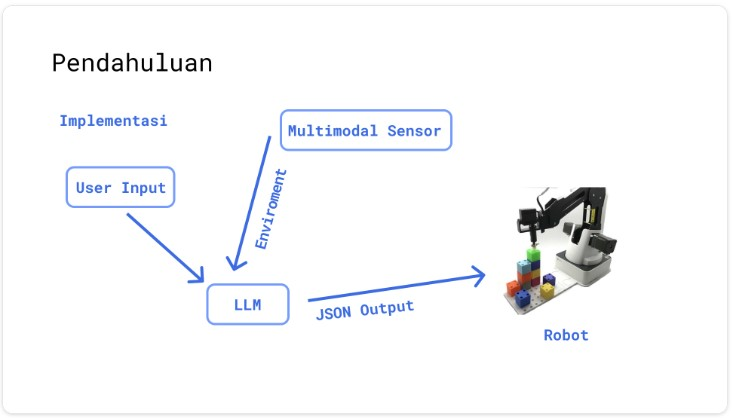
\includegraphics[scale=0.8]{gambar/pend.jpg}
  % Keterangan gambar yang diinputkan
  \caption{Alur sistem}
\end{figure}

Metode yang digunakan untuk menyelesaikan tugas akhir ini dapat diuraikan sebagai berikut. Pertama-tama, sistem akan menerima input dari berbagai sumber, termasuk sensor multimodal yang menggunakan kamera dengan OpenCV untuk mendeteksi objek dalam lingkungan sekitar. Informasi kontekstual juga diperoleh, mencakup fungsi yang dapat diakses oleh robot (misalkan fungsi "gerak()") serta tujuan kontrol yang diinginkan oleh pengguna (misalkan "ambil balok merah"). Selajutnya dengan memanfaatkan teknologi model bahasa besar, sistem memproses seluruh input yang diberikan untuk menghasilkan rencana aksi bagi robot. Pada tahap terakhir, output melibatkan konversi hasil rencana tersebut ke dalam format JSON. Format ini digunakan untuk menyusun serangkaian instruksi yang dapat diinterpretasikan oleh robot. Dengan menggunakan Dobot API Python, informasi tersebut diubah menjadi gerakan Dobot yang dapat dieksekusi oleh robot sesuai dengan aksi yang telah ditetapkan. Dengan mengikuti langkah-langkah ini, sistem mampu menerima instruksi dari pengguna, memahaminya, dan menerjemahkannya menjadi tindakan yang dapat dilakukan oleh robot dalam lingkungan sekitarnya.

\section{Metode}

\textit{}

Metode yang diterapkan untuk menyelesaikan tugas akhir ini telah dirancang dengan langkah-langkah yang terperinci untuk memastikan keberhasilan proyek. Tahap pertama adalah pengumpulan dataset, di mana data yang relevan dikumpulkan dalam bentuk pasangan masukan dan keluaran untuk digunakan dalam proses pengembangan model. Selanjutnya, proses finetuning dilakukan, di mana model bahasa disesuaikan dengan dataset baru yang telah terkumpul, memastikan bahwa model mampu mengenali pola-pola dalam data yang bersangkutan. Setelah itu, evaluasi metrik menjadi langkah krusial dalam memeriksa performa model yang telah disesuaikan. Dengan menggunakan metrik evaluasi, hasil dari model dievaluasi untuk menentukan seberapa baik model dapat menghasilkan output yang diinginkan. Apabila hasil evaluasi masih belum memenuhi target yang telah ditetapkan, maka dilakukan iterasi kembali pada tahap pengumpulan dataset atau finetuning. Dengan pendekatan ini diharapkan bahwa proyek tugas akhir ini akan menghasilkan model yang optimal dan sesuai dengan kebutuhan yang diinginkan.


\begin{figure} [H] \centering
  % Nama dari file gambar yang diinputkan
  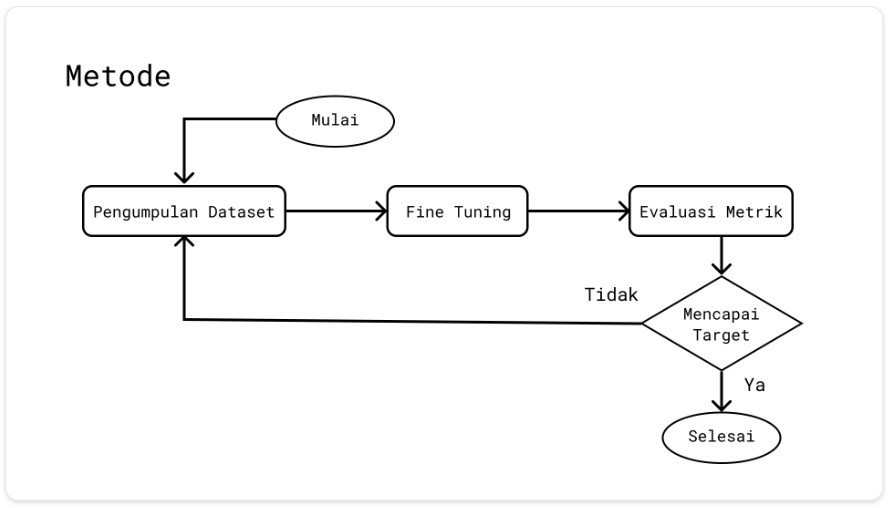
\includegraphics[scale=0.7]{gambar/metode.jpg}
  % Keterangan gambar yang diinputkan
  \caption{Metode}
\end{figure}


\section{Dataset}
Dalam pengembangan model untuk pengendalian robot, jenis dataset yang digunakan memiliki peran yang penting dalam memperkuat kemampuan sistem. Pertama, jenis dataset \textit{Direct Command} digunakan untuk melatih model dalam mengakses fungsi dasar robot dengan instruksi langsung. Dataset ini membantu model memahami dan mengeksekusi perintah-perintah dasar dengan akurat. Kedua, dataset \textit{Chain of Command} memberikan latihan pada model untuk mengakses beberapa fungsi dasar robot secara bersamaan, memungkinkan robot untuk melakukan serangkaian tindakan terkait dengan satu instruksi. Selanjutnya, dataset \textit{Reasoning}menekankan pada pelatihan model untuk menentukan rencana tindakan terbaik untuk mencapai tujuan pengguna tanpa adanya instruksi yang eksplisit. Dengan demikian, model diajarkan untuk memahami konteks dan tujuan yang lebih luas dalam mengambil keputusan. Terakhir, kriteria terakhir adalah dataset \textit{Impossible Task}, di mana model diuji dengan permintaan yang tidak sesuai dengan batasan lingkungan. Dalam situasi ini, model harus dapat mengenali batasan tersebut dan mengembalikan error sebagai respons yang tepat.



\begin{figure} [H] \centering
  % Nama dari file gambar yang diinputkan
  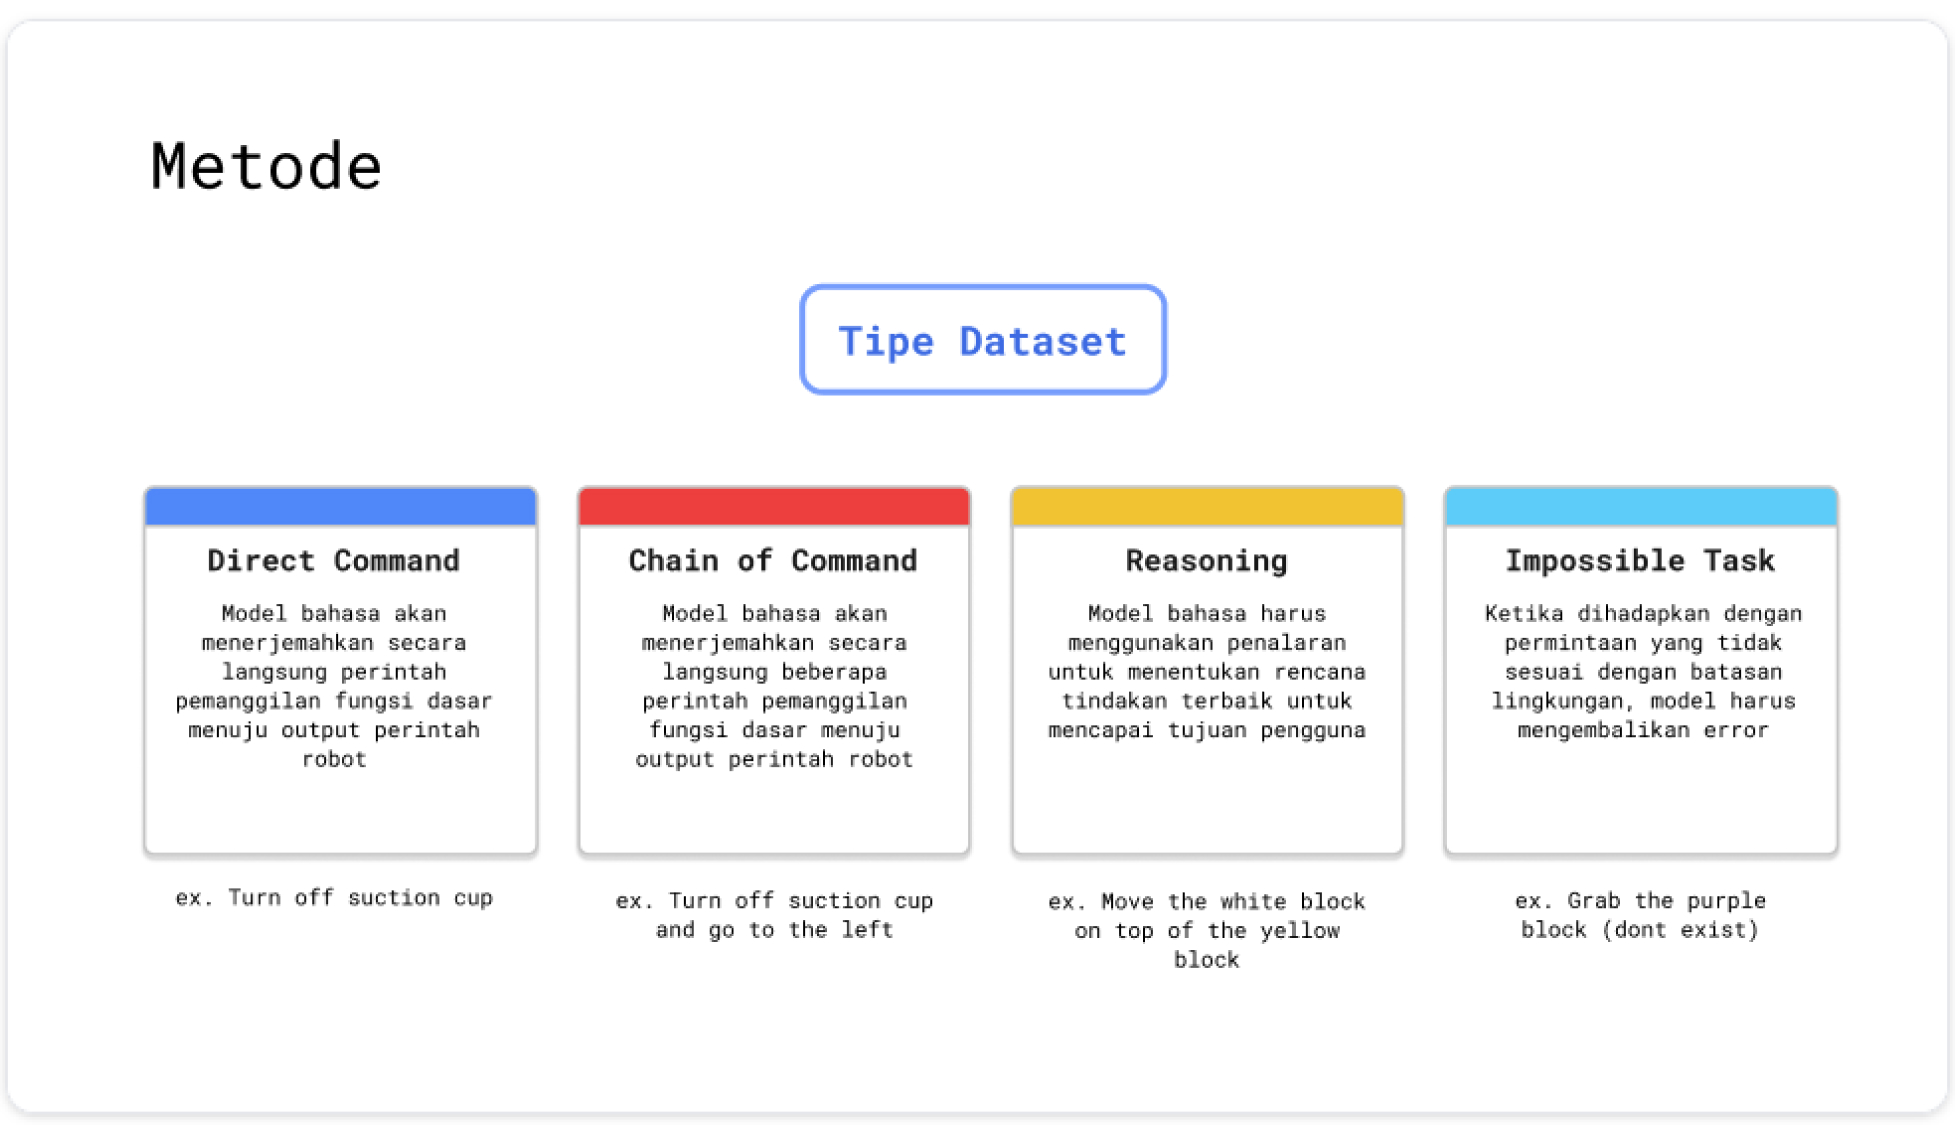
\includegraphics[scale=0.17]{gambar/tip_dat.jpg}
  % Keterangan gambar yang diinputkan
  \caption{Kriteria Dataset}
\end{figure}

\begin{figure} [H] \centering
  % Nama dari file gambar yang diinputkan
  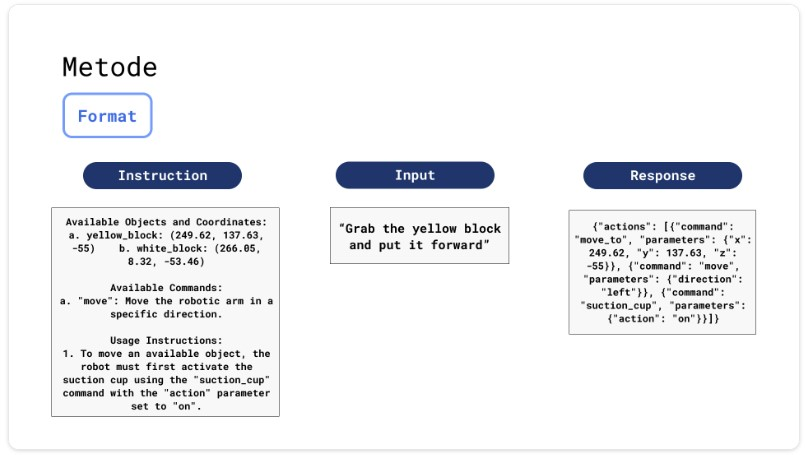
\includegraphics[scale=0.7]{gambar/format-data.jpg}
  % Keterangan gambar yang diinputkan
  \caption{Format Dataset}
\end{figure}

Untuk proses fine-tuning, format dataset akan disusun sesuai dengan format Alpaca Stanford, yang memiliki komponen-komponen sebagai berikut. Bagian \textit{Instruction} berisi instruksi yang diperlukan untuk mencapai output yang diinginkan. Dalam penelitian ini, instruksi mencakup kondisi nyata lingkungan seperti objek yang dapat dimanipulasi dan koordinatnya. Selain itu, terdapat pula fungsi dasar yang dapat diakses oleh model bahasa (misalkan fungsi Gerak()) yang digunakan untuk mengendalikan robot. Instruksi penggunaan juga disertakan, yang berisi langkah-langkah yang harus diambil untuk mencapai keluaran yang diharapkan. Bagian \textit{Input} berisi perintah yang diberikan oleh pengguna kepada robot. Contohnya, perintah untuk "mengambil blok merah dan memindahkannya ke depan". Bagian \textit{Output} berisi hasil keluaran berupa rencana aksi robot dalam format JSON. Rencana ini mencakup langkah-langkah yang harus dilakukan oleh robot berdasarkan instruksi yang diberikan dan kondisi lingkungan yang ada. Dengan menyusun dataset dalam format ini, proses fine-tuning dapat dilakukan dengan lebih terstruktur dan memungkinkan model untuk belajar dengan lebih efektif dari interaksi antara pengguna dan robot.



\section{\textit{Fine Tuning}}

\begin{figure} [H] \centering
  % Nama dari file gambar yang diinputkan
  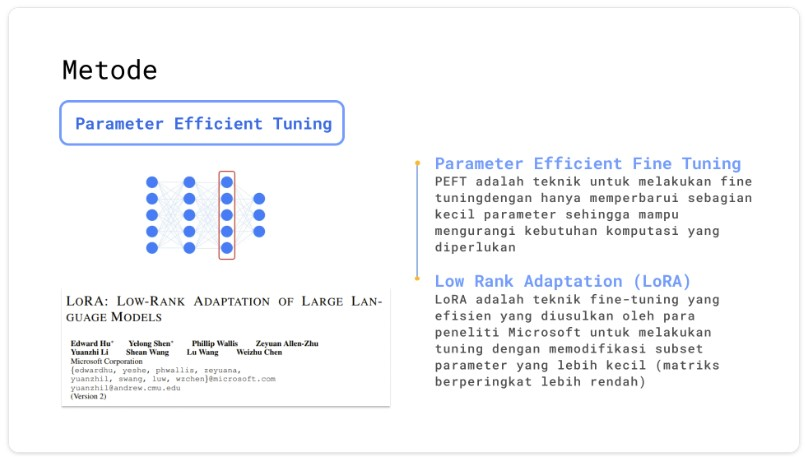
\includegraphics[scale=0.7]{gambar/lora_tun.jpg}
  % Keterangan gambar yang diinputkan
  \caption{Tuning}
\end{figure}

  Proses \textit{fine tuning} melibatkan penyesuaian model bahasa yang telah ada dengan dataset yang spesifik atau tugas yang diinginkan. Tujuan utamanya adalah untuk meningkatkan kemampuan model bahasa dalam menangani tugas atau lingkungan yang lebih spesifik dengan lebih baik. Dalam penelitian ini, \textit{fine tuning} bertujuan agar model bahasa menghasilkan rencana aksi robot yang optimal berdasarkan instruksi pengguna dan parameter pendukung. Dengan ini, kemampuan robot untuk merespons dan berinteraksi dengan lingkungan sekitarnya dengan lebih efektif. Seiring dengan peningkatan kinerja model, harapannya adalah bahwa robot akan mampu melakukan tugas-tugas yang kompleks dengan lebih baik dan menghasilkan rencana aksi yang lebih tepat sesuai dengan kebutuhan dan preferensi pengguna.


\section{Evaluasi Metrik}

\begin{figure} [H] \centering
  % Nama dari file gambar yang diinputkan
  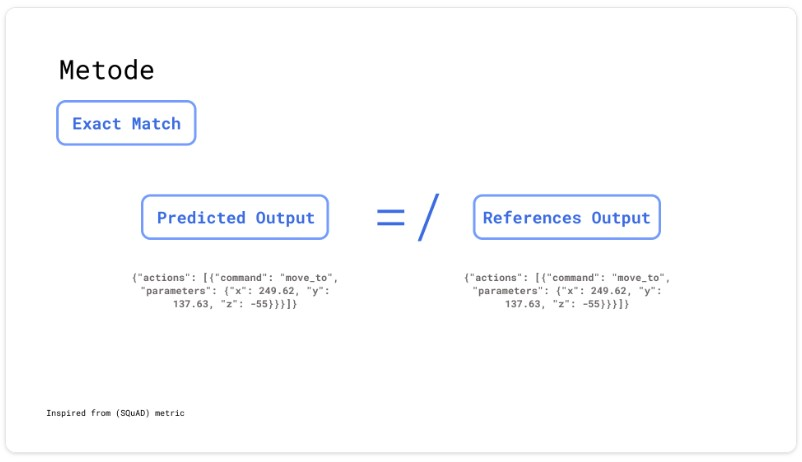
\includegraphics[scale=0.7]{gambar/exact.jpg}
  % Keterangan gambar yang diinputkan
  \caption{Metrik \textit{Exact Match}}
\end{figure}

Dalam penelitian ini, metrik \textit{exact match} dipilih sebagai metrik evaluasi. Pendekatan ini menilai kinerja model dengan membandingkan secara langsung antara output prediksi model dengan label atau output yang seharusnya sesuai. Metrik ini dipilih didasarkan pada fakta bahwa output yang dihasilkan oleh model berbentuk JSON, sebuah format yang struktural dan tidak dalam bentuk bahasa alami. Oleh sebab itu, penggunaan metrik \textit{exact match} menjadi relevan karena memungkinkan evaluasi yang langsung terhadap kesesuaian antara output model dengan label yang diharapkan dalam format JSON yang terstruktur. Dengan memastikan kesesuaian ini, kami dapat memastikan bahwa respons yang dihasilkan oleh model sesuai dengan aksi yang diinginkan untuk robot berdasarkan kondisi yang diberikan.



